\selectlanguage{english}%

\chapter{Decidibilità Delle Logiche Modali}


\section{Filtrazione}

Dato una logica $\Lambda$ e una formula a, si può garantire cheesiste
un modello $\mu$, con un numerodi mondi limitato da f(n), con n numero
di sottoformule di a tale che:

$\teoremaDi{\Lambda}a\iff\vera{\mu}a$

Dimostrazione.

Ip) $a\in\Gamma\implies sottoformule(a)\subseteq\Gamma$

Ts) $\exists\mu:\,\teoremaDi{\Lambda}a\iff\vera{\mu}a$

sia $\mu$=(S,R,V), consideriamo la seguente relazione:

$\sim_{\Gamma}\subseteq S\times S$

che gode della seguente proprietà:

$\Gamma_{\alpha}=\{a\in\Gamma\,|\,\veraw{\mu}{\alpha}a\}$

$\alpha\sim_{\Gamma}\beta\iff\Gamma_{\alpha}=\Gamma_{\beta}$

Si può notare che $\sim_{\Gamma}$ è una relazuione di equivalenza,
Infatti:
\begin{enumerate}
\item è simmetrica\\
$\alpha\sim_{\Gamma}\alpha\iff\Gamma_{\alpha}=\Gamma_{\alpha}$
\item è riflessiva\\
$\alpha\sim_{\Gamma}\beta\iff\Gamma_{\alpha}=\Gamma_{\beta}\iff\beta\sim_{\Gamma}\alpha$
\item è transitiva:\\
$\alpha\sim_{\Gamma}\beta\wedge\alpha\sim_{\Gamma}\gamma\iff\Gamma_{\alpha}=\Gamma_{\beta}=\Gamma_{\gamma}\iff\gamma\sim_{\Gamma}\beta$
\end{enumerate}
Posso allora considerare l'insieme quoziente:

$S_{\Gamma}=S/\sim_{\Gamma}$

Si può dimostrare con il teorema di fattorizzazzione delle applicazioni
che:

$|S_{\Gamma}|\leq2^{|\Gamma|}$

\begin{center} 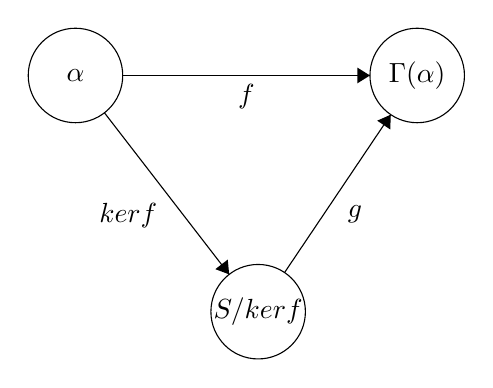
\begin{tikzpicture}[scale=0.2] \tikzstyle{every node}+=[inner sep=0pt] \draw [black] (22.1,-16.4) circle (3); \draw (22.1,-16.4) node {$\alpha$}; \draw [black] (43.8,-16.4) circle (3); \draw (43.8,-16.4) node {$\Gamma(\alpha)$}; \draw [black] (33.7,-31.4) circle (3); \draw (33.7,-31.4) node {$S/kerf$}; \draw [black] (35.38,-28.91) -- (42.12,-18.89); \fill [black] (42.12,-18.89) -- (41.26,-19.27) -- (42.09,-19.83); \draw (39.36,-25.24) node [right] {$g$}; \draw [black] (25.1,-16.4) -- (40.8,-16.4); \fill [black] (40.8,-16.4) -- (40,-15.9) -- (40,-16.9); \draw (32.95,-16.9) node [below] {$f$}; \draw [black] (23.94,-18.77) -- (31.86,-29.03); \fill [black] (31.86,-29.03) -- (31.77,-28.09) -- (30.98,-28.7); \draw (27.33,-25.31) node [left] {$kerf$}; \end{tikzpicture} \end{center}

Per dimostrarlo basta prendere:

$f:\,\alpha\rightarrow\mathcal{P}(\Gamma)$

risulta banale verificare che:

$ker\, f\equiv\sim_{\Gamma}$

e quindi, ricordando che g è iniettiva, risulta banale che:

$|S/\sim_{\Gamma}|\leq\Gamma(\alpha)$

Allora possiamo prendere il modello:

$M^{\Gamma}=(S^{\Gamma},R',V^{\Gamma})$

$R'\subseteq S^{\Gamma}\times S^{\Gamma}$

con R' che soddisfi le seguenti proprietà:

F1) $(\alpha,\,\beta)\in R\implies([\alpha],\,[\beta])\in R'$

F2) $([\alpha],[\beta])\in R'\implies\forall\boxx b\in\Gamma,\,\veraw{\mu}{\alpha}{\boxx b}\implies\veraw{\mu}{\beta}b$

Una relazione che gode delle proprietà F1 e F2 si chiama $\Gamma$-filtrazione
della relazione R.

prendiamo infine:

$V^{\Gamma}:\,\Phi\cap\Gamma\rightarrow\mathcal{P}(S^{\Gamma})$

che gode della seguente proprietà:

presa una formula atomica $A\in\Phi\cap\Gamma$

$\alpha\in V^{\Gamma}(A)\iff\alpha\in V(A)$


\subsection{Teorema}

Esiste almeno una relazione che gode delle proprietà F1 e F2:

$R^{\sigma}\subseteq S^{\Gamma}\times S^{\Gamma}$

così definita:

$([\alpha],[\beta])\in R^{\sigma}\iff\exists\delta\in[\alpha],\eta\in[\beta]\,:\,(\delta,\,\eta)\in R$

La proprietà F1 è dimostrata banalmente.

Dimostriamo F2

Ip) $([\alpha],[\beta])\in R^{\sigma}$, $\boxx{b\in\Gamma}$, $\veraw{\mu}{\alpha}{\boxx b}$

Ts) $R^{\delta}$gode della proprietà F2

supponiamo che:

$\exists\delta,\eta\,:\,\delta R\eta\wedge\delta\in[\alpha]\wedge\eta\in[\beta]$

avremo che:

$\veraw{\mu}{\delta}{\boxx b}$

$\veraw{\mu}{\eta}b$

e quindi:

$\veraw{\mu}{\beta}b$\\



\section{Lemma di Filtrazione}

dato un insieme$\Gamma$ chiuso rispetto alle sottoformule di a, con
$a\in\Gamma$

$\veraw{\mu}{\alpha}{a\iff}\veraw{\mu^{\Gamma}}{\alpha}a$

per ogni $\mu^{\Gamma}$$\Gamma$-filtrazione di $\mu$

Dimostrazione:

Ts) $\veraw{\mu}{\alpha}{a\iff}\veraw{\mu^{\Gamma}}{[\alpha]}a$

Ip) $\mu^{\Gamma}$$\Gamma$-filtrazione di $\mu$

Per induzione sul numero di connettivi di a

Caso Base, n=0:

a non ha connettivi, allora $a\equiv A$

$\veraw{\mu}{\alpha}A\iff\alpha\in V(A)\iff\alpha\in V^{\Gamma}(A)\iff\veraw{\mu^{\Gamma}}{[\alpha]}a$

Ipotesi di induzione: il teorema vale per ogni formula di $\Gamma$
con m<n connettivi.

a può essere:
\begin{enumerate}
\item $\neg b$
\item $b\implies c$
\item $\boxx b$
\end{enumerate}
Caso 1:

$\veraw{\mu}{\alpha}{\neg b}\iff\nonveraw{\mu}{\alpha}b\iff\nonveraw{\mu^{\Gamma}}{[\alpha]}b\iff\veraw{\mu^{\Gamma}}{[\alpha]}{\neg b}$

Caso 2:

$\veraw{\mu}{\alpha}{b\implies c}$ se e solo se $\nonveraw{\mu}{\alpha}b$
oppure $\veraw{\mu}{\alpha}c$

quindi si può affermare

$\nonveraw{\mu}{\alpha}b\iff\nonveraw{\mu^{\Gamma}}{[\alpha]}b$

$\veraw{\mu}{\alpha}c\iff\veraw{\mu^{\Gamma}}{[\alpha]}c$

ma vale almeno una delle due se e solo se

$\veraw{\mu^{\Gamma}}{[\alpha]}{b\implies c}$

Caso 3:

Ip) $\veraw{\mu}{\alpha}{\boxx b}$

Ts) $\veraw{\mu^{\Gamma}}{[\alpha]}{\boxx b}$

Consideriamo la reazione R' avente le proprietà F1 e F2

$\forall[\beta]\,:\,([\alpha],\,[\beta])\in R'\implies\veraw{\mu^{\Gamma}}{[\beta]}b$
-- per F2

allora si può affermare che:

$\veraw{\mu}{\beta}b\implies\veraw{\mu^{\Gamma}}{[\beta]}b\implies\veraw{\mu^{\Gamma}}{[\alpha]}{\boxx b}$

Ip)$\veraw{\mu^{\Gamma}}{[\alpha]}{\boxx b}$

Ts)$\veraw{\mu}{\alpha}{\boxx b}$

$\forall[\beta]\,:\,(\alpha,\,\beta)\in R,\,([\alpha],\,[\beta])\in R'$
--per F1

allora si può affermare che:

$\veraw{\veraw{\mu^{\Gamma}}{[\beta]}b\implies\mu}{\beta}b\implies\veraw{\mu}{\alpha}{\boxx b}$


\section{Determinatezza di K dai Frame Finiti}

La minima logica normale K è determinata dalla classe di tutti i frame
finiti.

Se $a$ ha n sottoformule $a$ è un teorema di K se e solo se A è
valida in tutti i frame con meno di $2^{n}$ mondi. 

$\teoremaDi Ka$ se e solo se $\vera Fa$.\\


Ip)$\teoremaDi Ka$ 

Ts)$\vera Fa$\\


Se $a$ è un teorema di K allora $a$ è valida in tutti i frame (infatti
K è determinata rispetto alla classe di tutti i frame) è a maggior
ragione valida in tutti i frame finiti ed in tutti i frame con meno
di $2^{n}$ mondi.\\


Ip)$\vera Fa$

Ts)$\teoremaDi Ka$\\
\\
Suppongo per assurdo che$\nonTeor Ka$ se e solo se $\nonvera{M^{K}}a$
se e solo se (per il lemma di filtrazione) $\nonvera{(M^{K})^{\Gamma}}a$
il che implica che

in particolare $\nonvera{(F^{K})^{\Gamma}}a$ dove $(F^{K})^{\Gamma}$
è il Frame su cui è costruita la filtrazione del modello canonico
costruito rispetto alla logica $K$ 

Si noti che $(M^{K})^{\Gamma}$ ha al più $2^{n}$ mondi.


\section{Determinatezza di KD dai Frame seriali finiti}

Per seguire lo stesso ragionamente della dimostrazione appena fatta,
dobbiamo solo mostrare che se $R$ è seriale allora $R^{\sigma}$
lo è.\\


\ovalbox{\begin{minipage}[t]{1\columnwidth}%
\textbf{Nota:}$R^{\sigma}\subseteq S^{\Gamma}\times S^{\Gamma}$

così definita:

$([\alpha],[\beta])\in R^{\sigma}\iff\exists\delta\in[\alpha],\eta\in[\beta]\,:\,(\delta,\,\eta)\in R$%
\end{minipage}}\\
\\
Sia $[\alpha]\in S^{\Gamma}$

Se $R^{KD}$ è seriale allora $\forall\delta\in S^{KD}\exists\eta\in S^{KD}:\ (\delta,\eta)\in R^{KD}$

In particolare esiste$\delta$ appartiene alla classe di equivalenza
$[\alpha]$ (di cui al limite potrebbe essere l'unico elemento con
$\alpha=\delta$)

Dalla serialità abbiamo che esiste$\eta$ appartiene alla classe di
equivalenza $[\beta]$

Da cui $([\alpha],[\beta])\in R^{\sigma}$


\section{Determinatezza di K4 dai Frame transitivi finiti}

L'aspetto interessante di questa dimostrazione sta nel fatto che non
possiamo usare la relazione ``classica'' $R^{\sigma}$ come $\Gamma$-filtrazione
ma dobbiamo costruirne una ad hoc, dato che se $R^{K4}$ è transitiva
la sua filtrazione standard non è detto che lo sia

Definiamo quindi $R^{\tau}$così:

$([\alpha],[\beta])\in R^{\tau}$ se se e solo se per ogni fbf $b$,
$\boxx b\in\Gamma$ e $\vera M{_{\alpha}\boxx b}$ implicano $\vera M{_{\beta}b\wedge\boxx b}$

dimostriamo che $R^{\tau}$ è una $\Gamma$-filtrazione transitiva\\


$R^{\tau}$è una $\Gamma$-filtrazione\\


F2) $([\alpha],[\beta])\in R^{\tau}$ se e solo se$\vera M{_{\alpha}\boxx b}$
implicano $\vera M{_{\beta}b\wedge\boxx b}$ da cui: $\{b\ |\ \boxx{b\in\alpha\}\subseteq\beta}$
e quindi $\alpha,\beta\in R^{K4}$

F1) $(\alpha,\beta)\in R^{K4}$per ogni $\boxx{b\in\Gamma}$, se $\vera M{_{\alpha}\boxx b}$
allora anche (schema 4) $\veraw M{\alpha}{\boxx{\boxx b}}$ 

dato che $(\alpha,\beta)\in R^{K4}$ , anche:

$\veraw M{\beta}b$ e $\veraw M{\beta}{\boxx b}$ e quindi:

$\veraw M{\beta}{b\wedge\boxx b}$\\


$R^{\tau}$ è transitiva\\


Sia $([\alpha],[\beta])\in R^{\tau}$, $([\beta],[\gamma])\in R^{\tau}$
ora la prima implica che per ogni fbf $b$, da $\boxx{b\in\Gamma}$
e $\veraw M{\alpha}{\boxx b}$ segua $\vera M{_{\beta}\boxx{b\wedge b}}$,
e da questa essendo $([\alpha],[\beta])\in R^{\tau}$, segue anche
$\vera M{_{\gamma}\boxx{b\wedge b}}$, cioè $([\beta],[\gamma])\in R^{\tau}$\selectlanguage{italian}%

